\documentclass{scrreprt}
\usepackage{array}
\usepackage{graphicx}
\usepackage{listings}
\usepackage{underscore}
\usepackage[bookmarks=true]{hyperref}
\usepackage[utf8]{inputenc}
\usepackage{float}
\usepackage[french]{babel}
\hypersetup{
    bookmarks=false,    % show bookmarks bar
    pdftitle={rapport_TP2_Lambolez_Petit},    % title
    pdfauthor={Théodore Lambolez, Maximilien Petit},                     % author
    pdfsubject={TeX and LaTeX},                        % subject of the document
    pdfkeywords={TeX, LaTeX, graphics, images}, % list of keywords
    colorlinks=true,       % false: boxed links; true: colored links
    linkcolor=blue,       % color of internal links
    citecolor=black,       % color of links to bibliography
    filecolor=black,        % color of file links
    urlcolor=black,        % color of external links
    linktoc=page            % only page is linked
}
\def\myversion{1.0}
\date{}
%\title
\usepackage{hyperref}
\begin{document}
\begin{figure}
   \begin{minipage}[c]{.46\linewidth}
      
\includegraphics[scale=0.3]{images/telecom.png}
   \end{minipage} \hfill
   \begin{minipage}[c]{.46\linewidth}
      
\includegraphics[scale=1.9]{images/lorraine.jpg}
   \end{minipage}
\end{figure}
\begin{flushright}
    \rule{15cm}{5pt}
    \vskip1cm
\end{flushright}
\begin{center}
	\vspace{3cm}
	\fbox{
	\begin{minipage}{0.9\textwidth}
        	\Huge{
			\textbf{
			\begin{center}
				Rapport \\Travaux Pratiques 2
				\vspace{0.5cm}
			\end{center}
			}
		}
	\end{minipage}
	}
\end{center}
\begin{flushright}
        \vspace{5cm}
	\huge{
        \textbf{
	Ecrit par \\
	\vspace{0,875cm}
	\href{mailto:theodore.lambolez@telecomnancy.eu}{Théodore Lambolez} \\
	\href{mailto:maximilien.petit@telecomnancy.eu}{Maximilien Petit}\\
	}
	}
        \vspace{0,5cm}
        \large{
	\textbf{
	\today\\
	}	
	}
\end{flushright}

\tableofcontents

\chapter{Introduction}

Ce deuxième travail pratique de Traitement Numérique de l'image fait suite à un travail d'initiation au logiciel
Optimas. L'objectif de ce deuxième, est de réaliser dans un premier temps un contrôle qualité automatiques de connecteurs. Puis, 
dans un second temps de réaliser une identification de dimension de clé. Sur ce même logiciel, il faudra donc cette fois-ci explorer
quelques pistes rendues possibles par sa fonctionnalité de création de "macros". On prendra soin tout au long de ce rapport, d'expliquer
les choix réalisés ainsi que leurs limites.


\chapter{Contrôle de la qualité des connecteurs}

\paragraph{Rappel de l'énoncé du problème traité :}
Nous sommes dans le cas où un industriel, par exemple, nous demande de réaliser un contrôle automatisé de la qualité des 
composants qui sortent à la fin de sa chaîne de production à l'aide de captures réalisées par un capteur spécifique.
Pour ce faire, il nous a fourni un échantillon de quelques captures de connecteurs parmi lesquelles on trouvera 
un témoin (ie. une capture de connecteur en bon état) ainsi que des captures de connecteurs présentant divers 
problèmes (broche pliée ou coupée, positionnement décentré et orientation diverse du connecteur).  

\paragraph{Stratégie adoptée :}
On se propose dans un premier temps d'étudier le problème du cas basique où le connecteur serait toujours placé
au même endroit sur l'image avec un même type de capteur qui serait situé à la même distance et dans les mêmes conditions 
environnementales (luminositée notamment). 

La stratégie adoptée dans ces conditions est alors de binariser l'image en choisissant un seuil qui permettrait
de ne mettre en valeur que les broches (fond en noir et objet en blanc). Ensuite, nous chercherons à caractériser un
cadre (ou R.O.I.) où chaque ligne de ce cadre passerait par les broches. De cette manière, en comptant pour un nombre
suffisamment grand de ligne avec un pas (sur l'axe des y) régulier entre ces lignes, on peut déterminer un pourcentage
de ligne passant par le bon nombre de broche (ici donné). Dans notre étude nous nous sommes fixé un seuil pour ce poucentage
qui nous permet de décider si l'état du connecteur est bon ou mauvais. Si le pourcentage est supérieur à 95% alors on peut 
estimer que le connecteur est en bon état. Dans le cas contraire, il serait en mauvais état. Cette valeur, 95%, est une valeur
définie arbitrairement qui pourrait être suceptible de changer suivant les améliorations qu'on pourrait faire de cette macro 
naïve.   

\paragraph{Travail préalable d'étude de l'échantillon d'image : }
Puisque nous avons choisi de réaliser une binarisation à partir d'un seuil à déterminer, nous avons réalisé 
une étude préalable des différentes façons de déterminer ce seuil. Nous avons rapidement conclus qu'il ne serait
pas forcément une bonne idée de réaliser un seuil fixe pour chaque image puisque la luminosité est une condition 
parfois difficile à maîtriser totalement. Nous choissons donc de déterminer un seuil calculé de manière dynamique
par optimas. Pour ce faire, Optimas proposes auto-threshold. On peut configurer cet outil pour qu'il réalise son 
calcule suivant différents critères. Sachant que nous ne voulons mettre en évidence que les broches, après avoir
essayé sur les échantillons données les différentes méthodes, nous avons convergé vers le calcul du seuil par 
minimisation de la variance. Néanmoins, une première limite se présente déjà. En effet, pour la capture prise 
dans des conditions de luminosité élevée, on remarque que d'autres parties que les broches du connecteur apparaissent
en blanc. Cela est dû au fait que la différence sur cette capture entre le niveau de gris des broches et le niveau de
gris du reste est trop faible. La méthode utilisée par l'au-threshold n'est donc pas suffisamment précise ici. 

Voici un échantillon des valeurs calculées pour chacune des captures de l'échantillon de base. 

\begin{table}[!h]
        \begin{center}
                \begin{tabular}{|c|c|c|}
                   \hline
                   Nom image & seuil bas & seuil haut \\
                   \hline
                   Connect1.tif & 110  & 255 \\
                   \hline
                   Connect2.tif & 116 & 255  \\
                   \hline
		   Connect3.tif & 116 & 255 \\
                   \hline 
		   Connect4.tif & 128 & 255 \\
                   \hline 
		   Connect5.tif & 126 & 255 \\
                   \hline 
		   Connect6.tif & 119 & 255 \\
                   \hline 
		   Connect7.tif & 124 & 255 \\
                   \hline 
		   Connect8.tif & 130 & 255 \\
                   \hline 
		   Connect9.tif & 129 & 255 \\
                   \hline 
		   Connect10.tif & 124 & 255 \\
		   \hline
 		   Connect11.tif & 126 & 255 \\
                   \hline
		   Connect12.tif & 129 & 255 \\
                   \hline 
 	
                \end{tabular}
        \end{center}
        \caption{Comparaison des seuils de binarisation automatique avec l'option de minimisation de la variance}
\end{table}

\paragraph{Analyse des résultats obtenu avec cette première macro : }
Voici quelques résultats obtenus avec la macro dont vous pourez trouver le script en annexe.

\begin{figure}[!h]
\centering
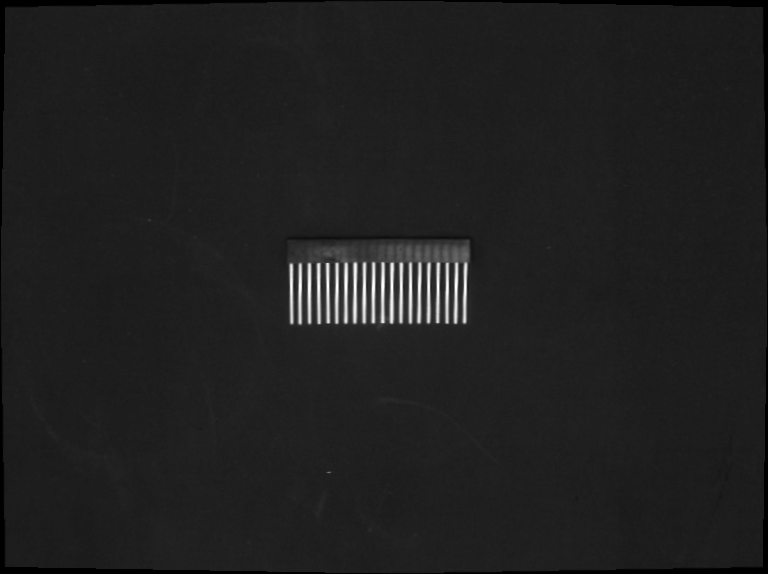
\includegraphics[width=5cm, height=5cm]{images/Connect1o.png}\hfill
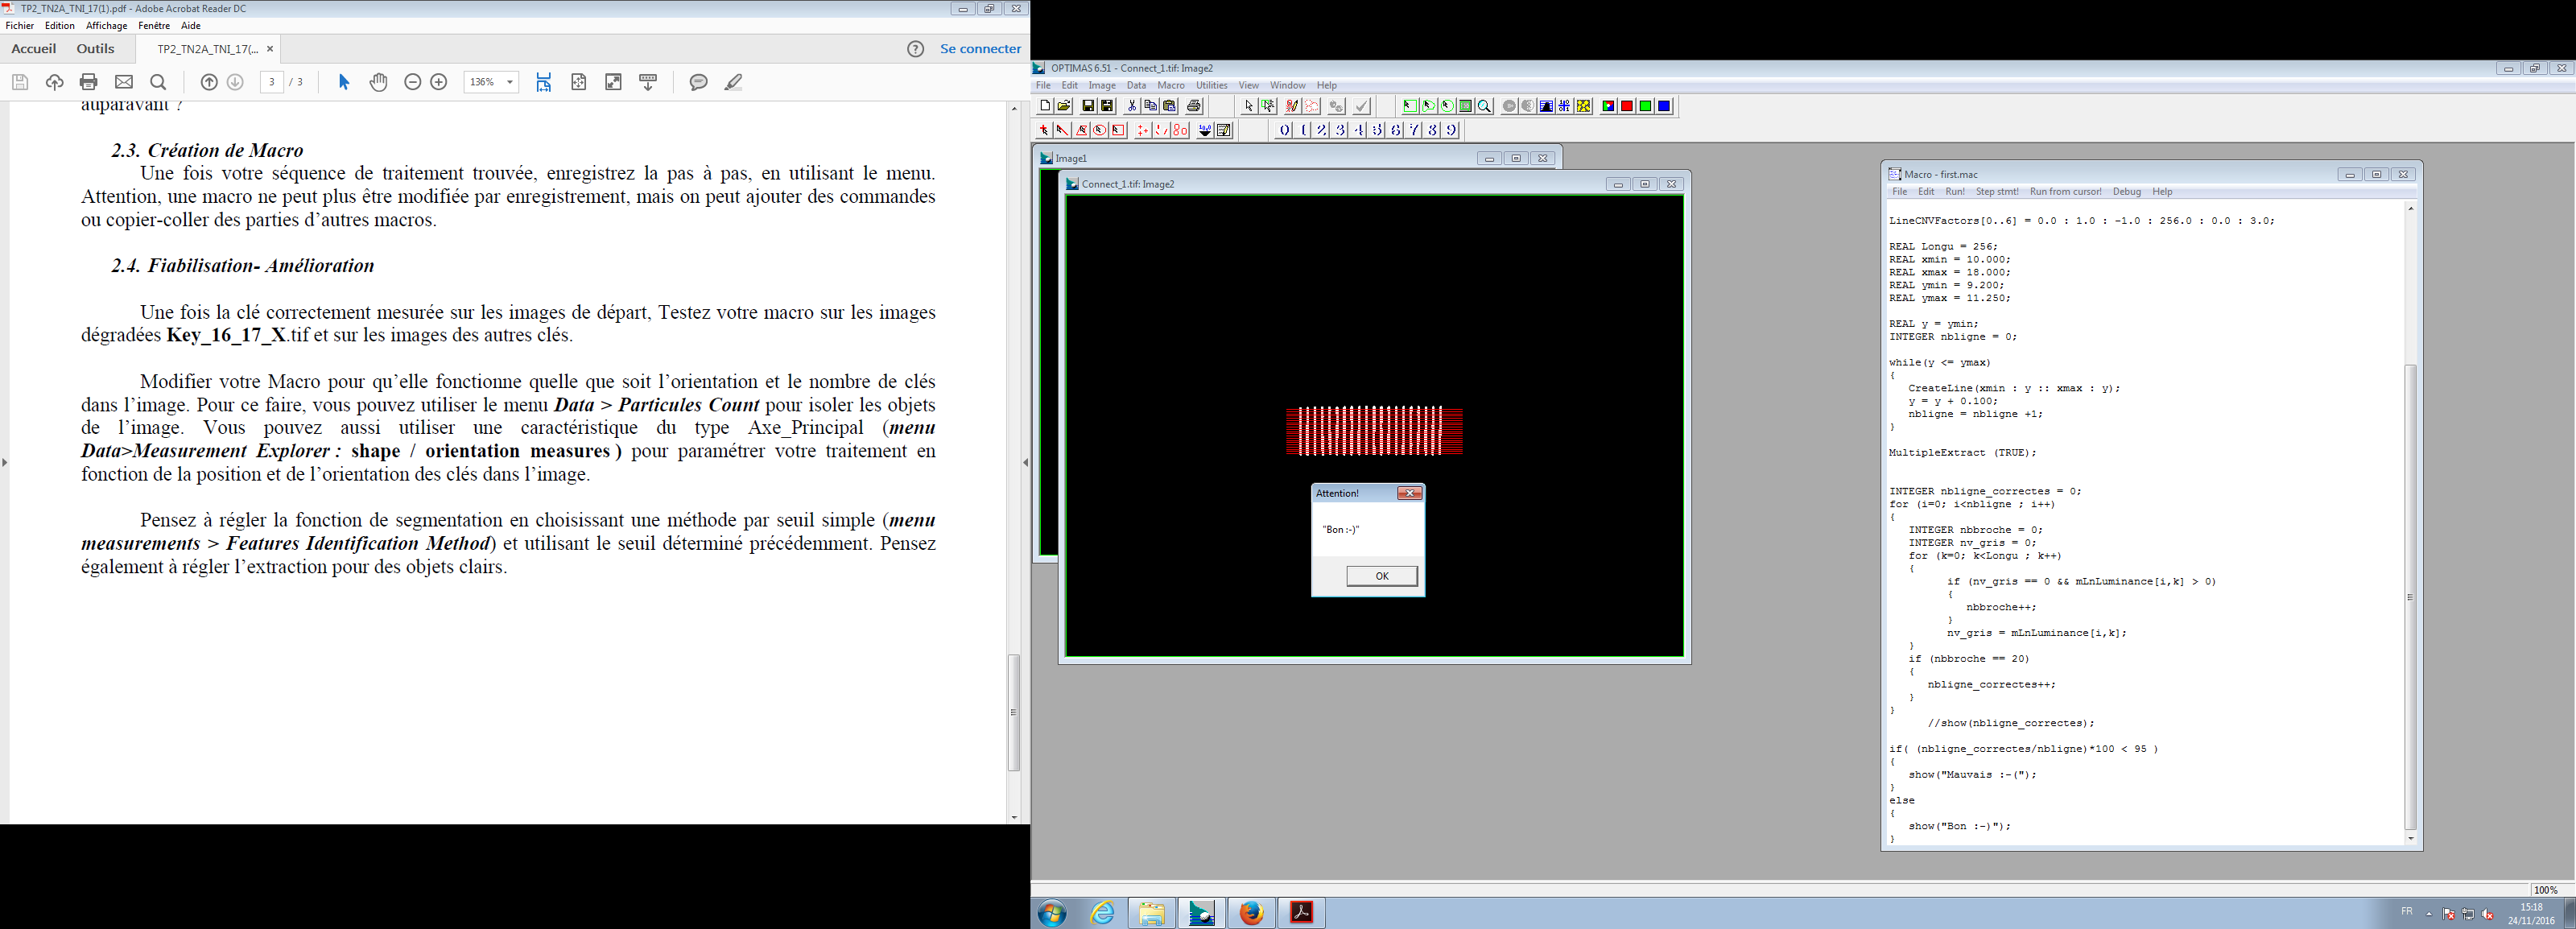
\includegraphics[width=5cm, height=5cm]{images/connecteur1.png}
\caption{Résultat de la macro pour l'image Connect_1.tiff}
\end{figure}

On constate heureusement que dans le cas de référence, la macro réalise correctement le travail souhaité. 

\newpage
\begin{figure}[!h]
\centering
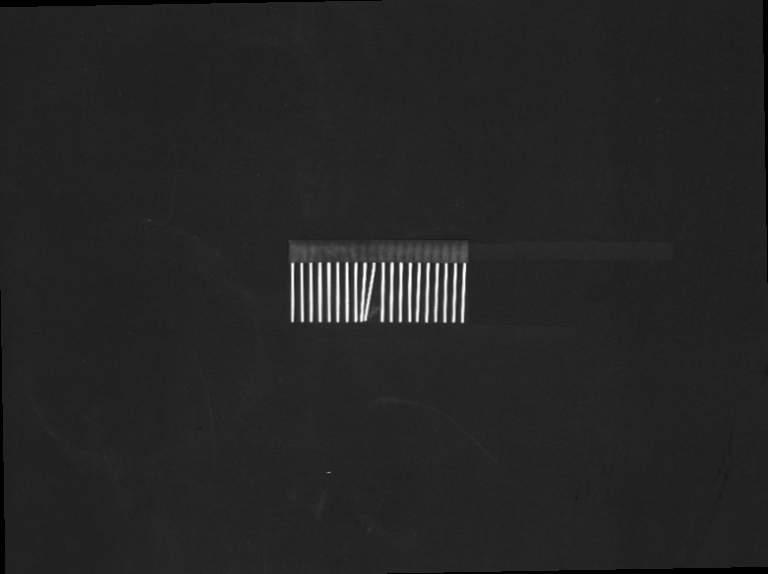
\includegraphics[width=5cm, height=5cm]{images/Connect2o.png}\hfill
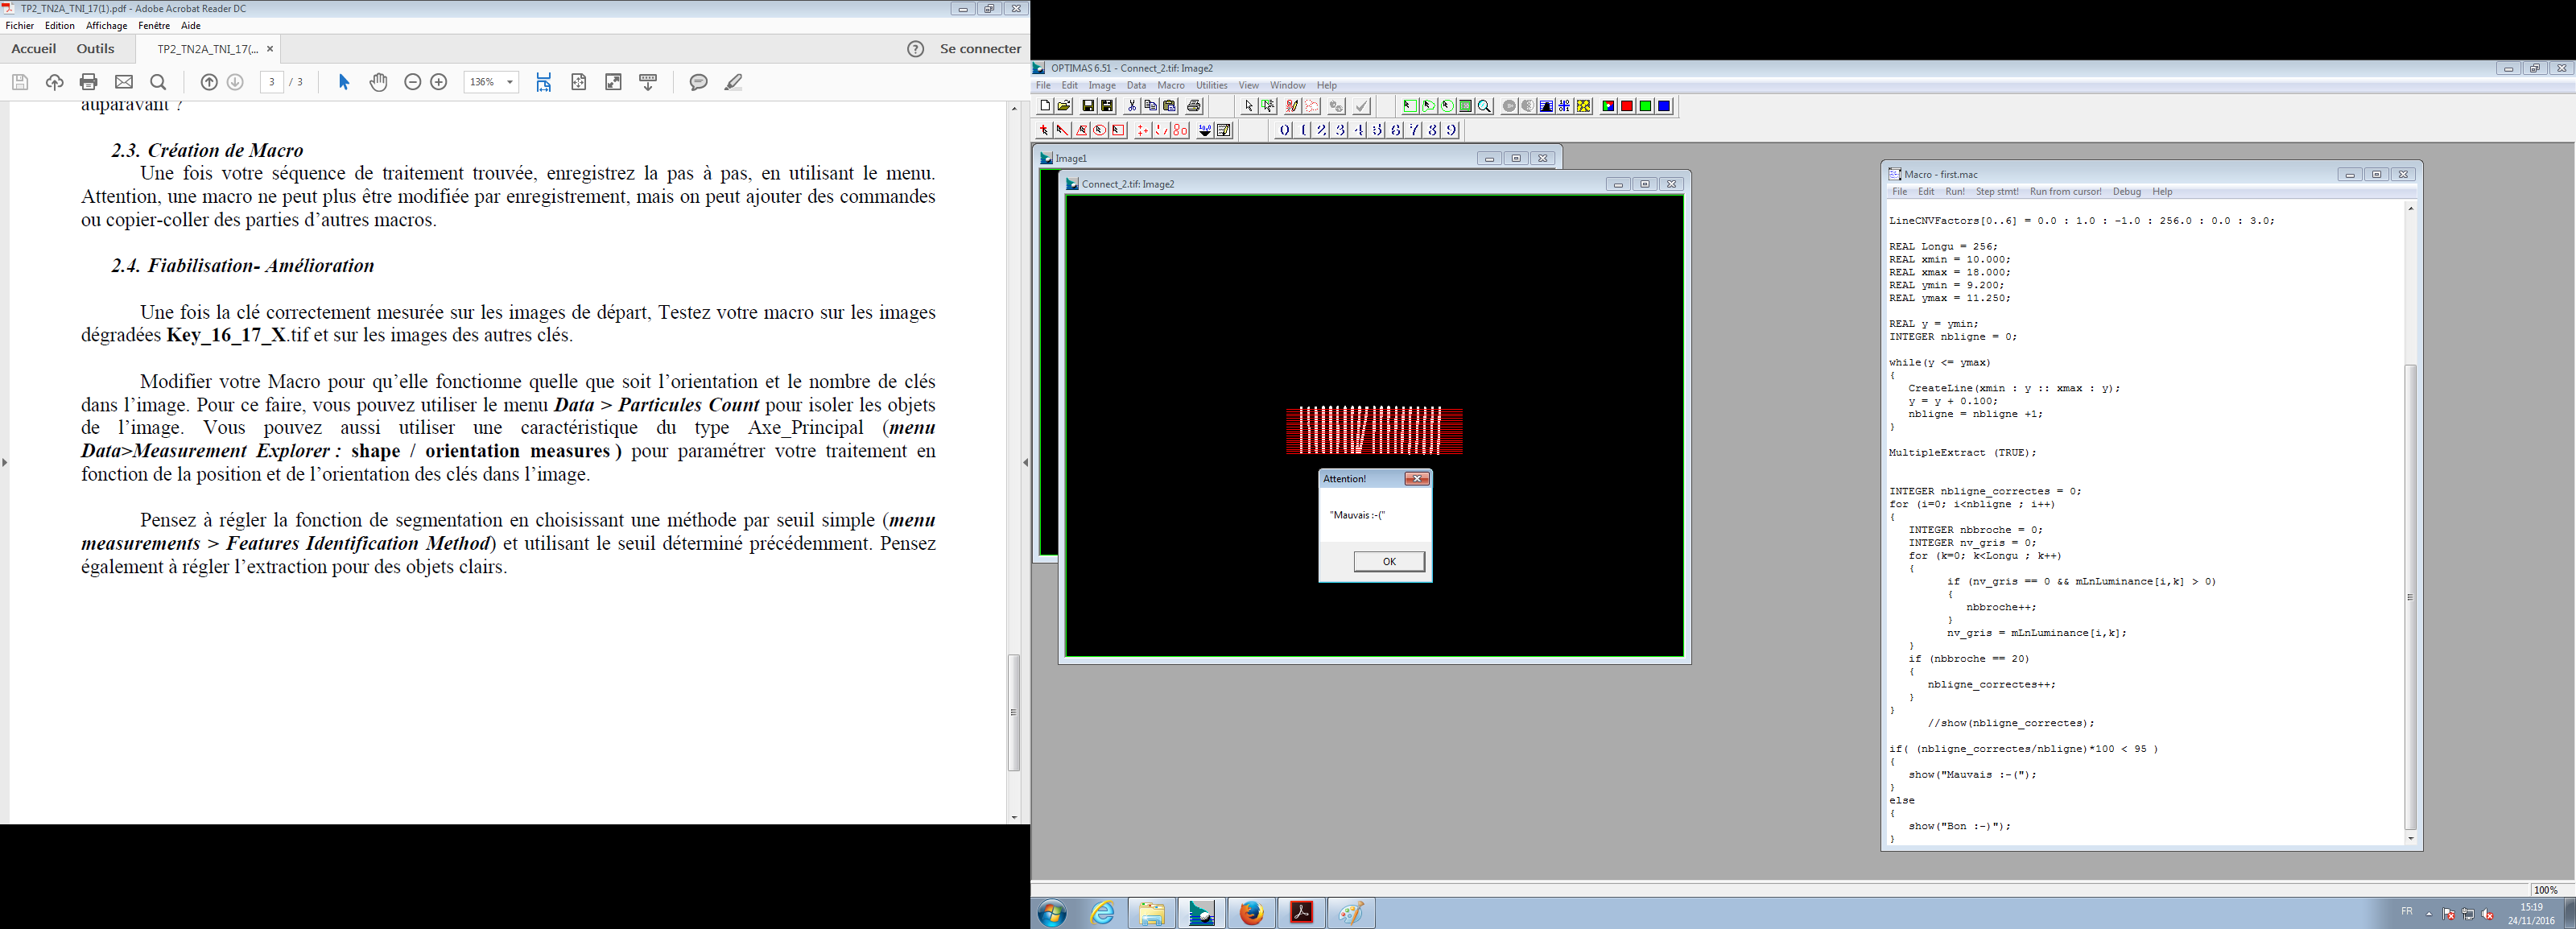
\includegraphics[width=5cm, height=5cm]{images/connecteur2.png}
\caption{Résultat de la macro pour l'image Connect_2.tiff}
\end{figure} 

On remarque dans ce deuxième cas où le connecteur est placé à la même position et présentant une broche pliée
que la macro considère que l'état est mauvais. En effet, à partir d'un moment, la broche pliée vient toucher 
une broche voisine. Puisque notre macro compte en fait les fronts montants des différents profils de lignes.
A partir de la hauteur de la capture où la broche vient toucher sa voisine, la macro ne comptera plus qu'un seul
front montant. 

Précision à propos du calcul du front montant. Nous avons choisi de garder en mémoire dynamiquement la valeur du niveau
de gris précédant lors du parcours du profil de ligne. De cette manière on peut comparer le niveau de gris précédant 
au niveau de gris courant. La condition de détection du front montant utilisé est en fait : si le niveau de gris précédant
est 0 (correspondant au noir du fond) et si le niveau de gris courant est strictement supérieur à 0, alors on a un front montant.

\begin{figure}[!h]
\centering
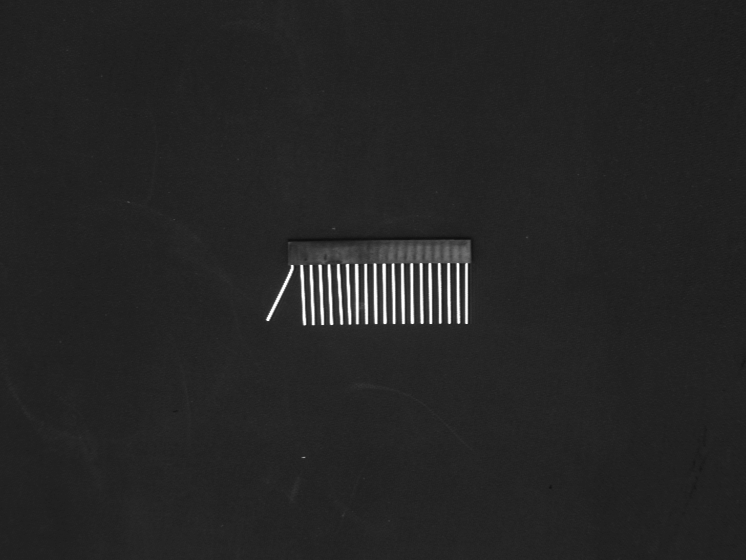
\includegraphics[width=5cm, height=5cm]{images/Connect3o.png}\hfill
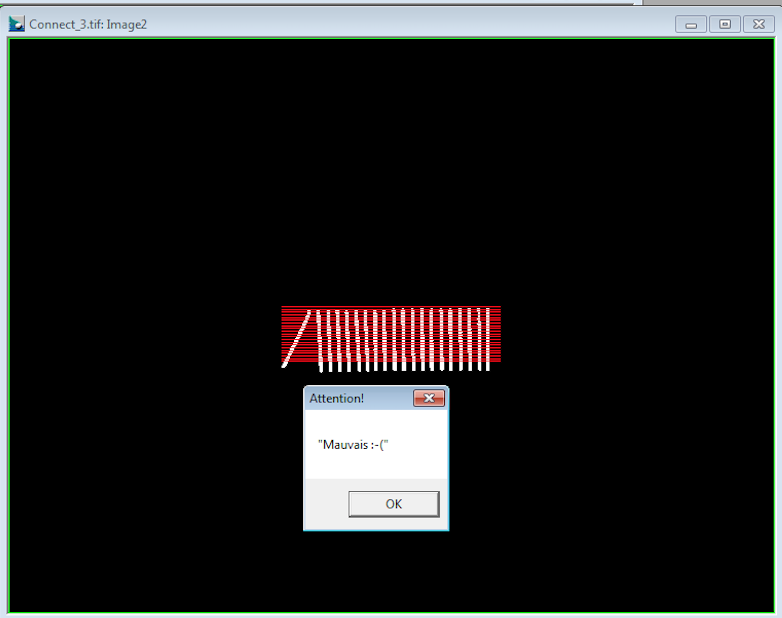
\includegraphics[width=5cm, height=5cm]{images/connecteur3.png}
\caption{Résultat de la macro pour l'image Connect_3.tiff}
\end{figure}

Nous avons ici enfin un cas intéressant à analyser pour nous donner une première piste d'amélioration de la macro. 
En effet, nous constatons que la macro aboutis au fait que le connecteur est mauvais. Ce qui est juste ! 
Néanmoins, on constate également que la première ligne n'est en fait pas prise en compte. Ce qui signifie
que la macro donne la bonne réponse pour une mauvaise raison. Ici le connecteur n'a pas exactement la même place 
sur la capture que le connecteur sur la capture de référence. Pour éviter ce problème, on peut réaliser une détection
de la position du premier pixel appartement à une broche. 

Une amélioration basique à réaliser serait de commencer par récupérer le nombre de pixel en largeur de l'image et de réaliser de cette
manière des profils de ligne (avec un pas très petit) successifs. On parcours chaque profil de ligne jusqu'à trouver un pixel blanc. 
On trouvera de cette manière le premier pixel appartenant à une broche du connecteur étudié. 

Un deuxième problème mis en évidence par ce test a été caché par le premier problème. En effet, même si le connecteur avait été à la bonne place
la macro aurait dit que le connecteur est bon. Il faut réduire la taille de la R.O.I fixée au début.

Une amélioration basique faisant suite à la première serait en fait de définir différents pas de manière empiriques. En effet, une fois qu'on a la 
position du premier pixel faisant parti d'une broche, on pourrait définir un pas minime en x décroissant. Ensuite, il nous faut caractériser le cadre
par trois autres points. Le premier point décalé d'un certains nombre de pixel vers les x croissant donne le deuxième. Le premier point décalé vers 
les y croissant donne le troisième point. Et finalement le troisième point décalé du même nombre de pixel que le deuxième point vers les x croissant donnera
le quatrième point. On a donc ici en suivant cette méthode trois nouveaux pas à définir. En restreignant la R.O.I., la broche pliée sortirait du champs et
le problème serait bien détecté !

\begin{figure}[!h]
\centering
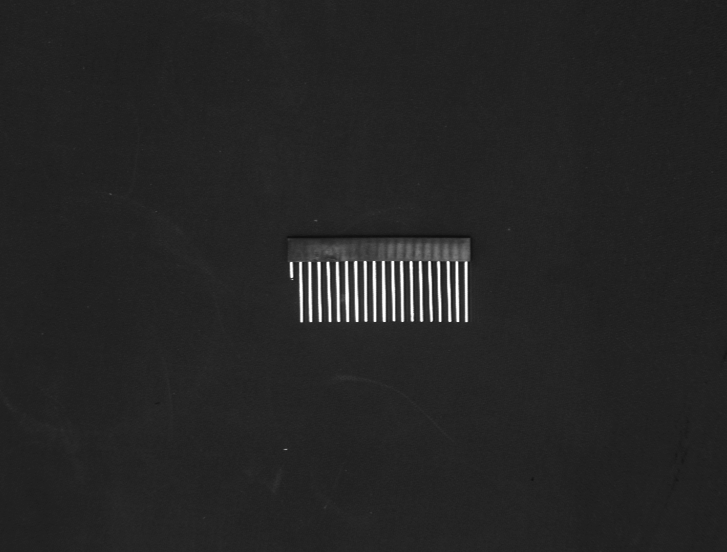
\includegraphics[width=5cm, height=5cm]{images/Connect4o.png}\hfill
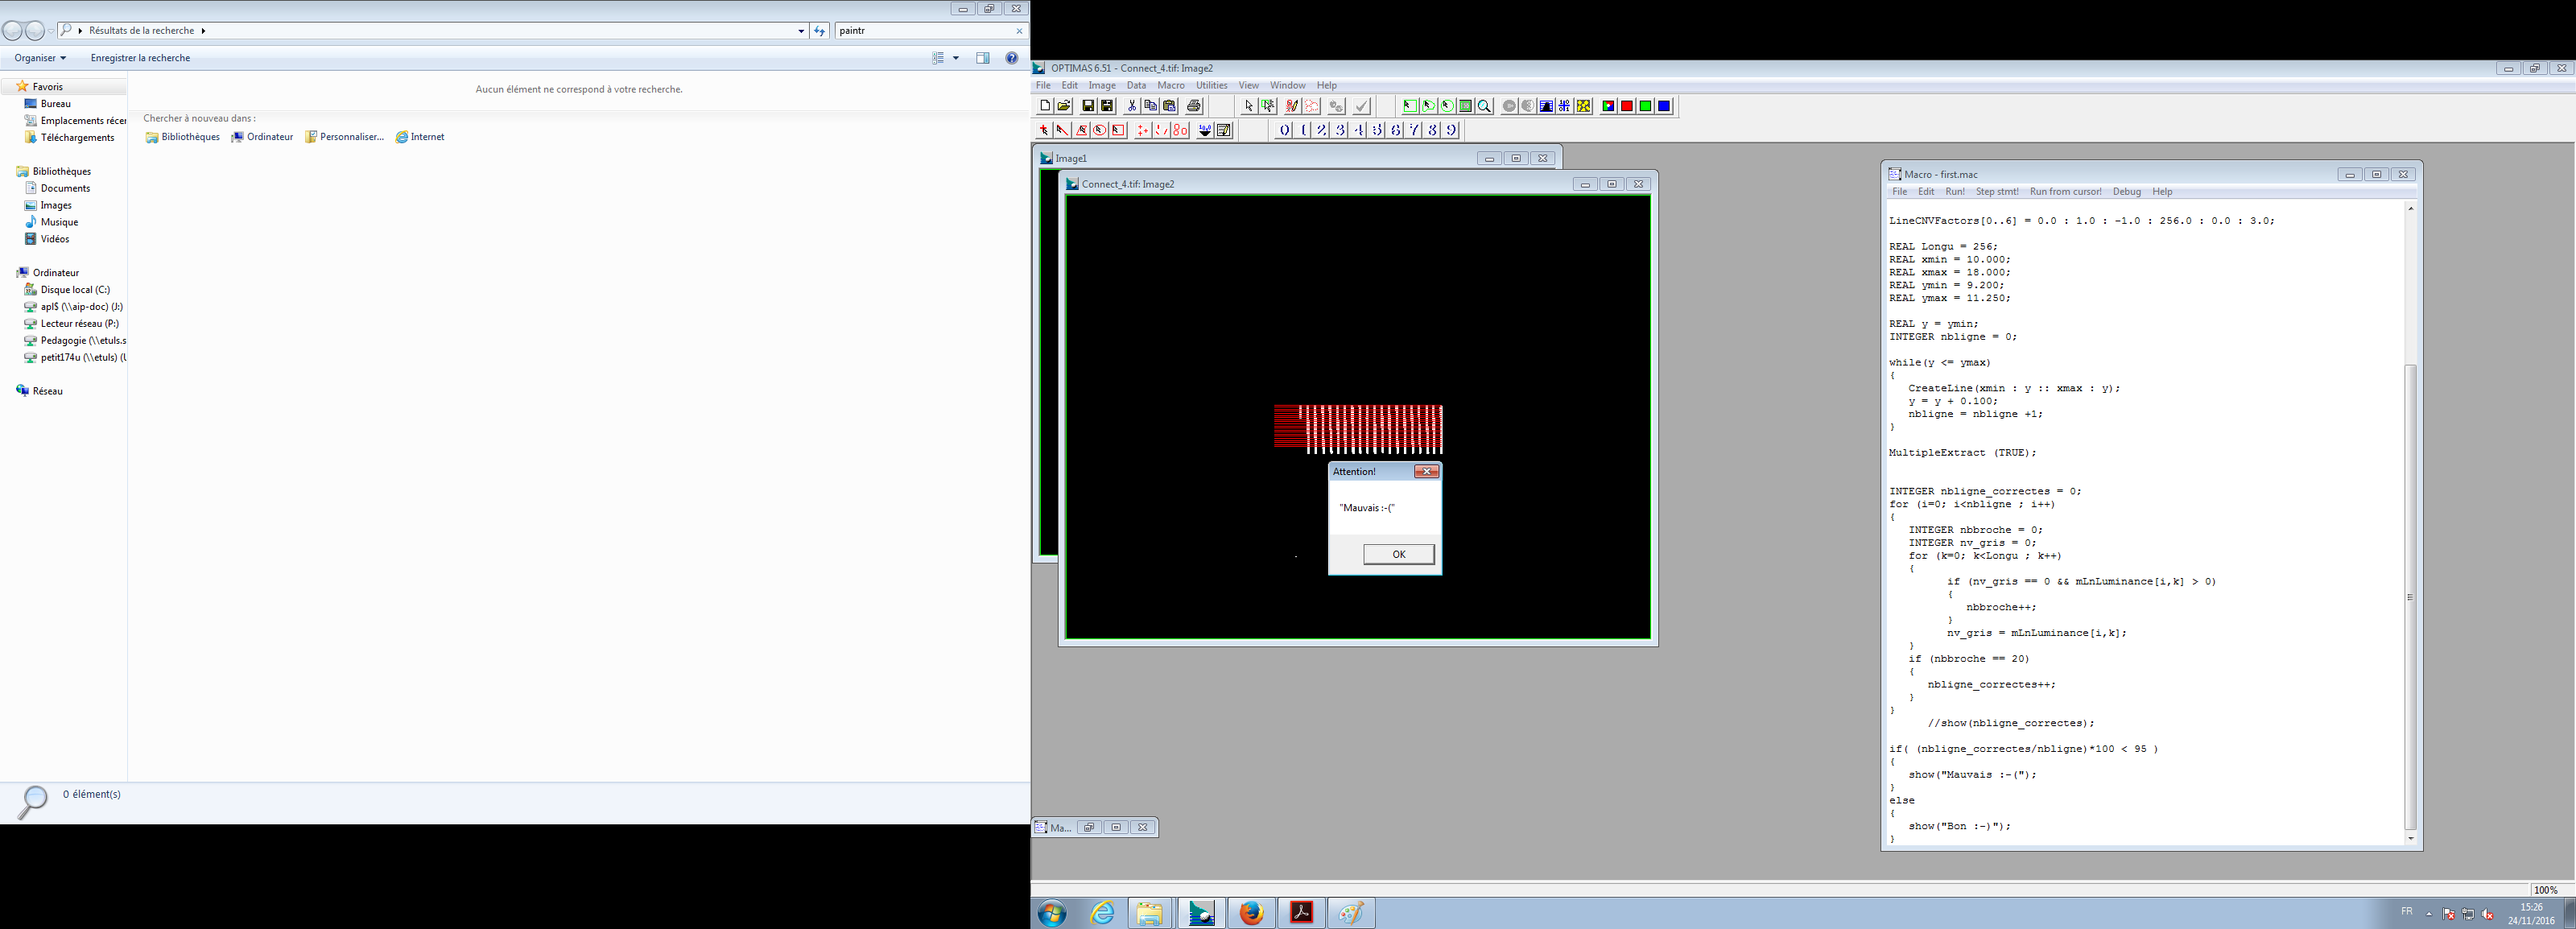
\includegraphics[width=5cm, height=5cm]{images/connecteur4.png}
\caption{Résultat de la macro pour l'image Connect_4.tiff}
\end{figure} 

Ici notre macro donne le bon résultat par chance. En effet, notre R.O.I. est un peu trop décalée par rapport aux broches du connecteur. L'amélioration
proposée précédemment permettrait d'éviter de jouer sur cette chance. 

\newpage
\begin{figure}[!h]
\centering
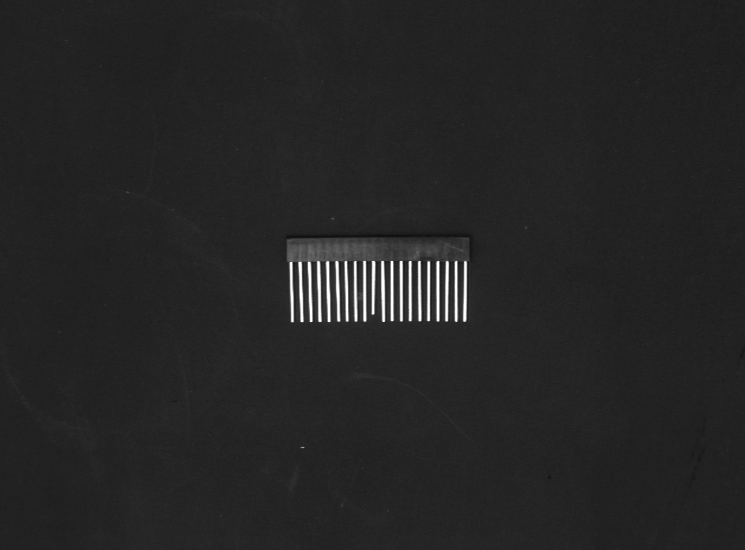
\includegraphics[width=5cm, height=5cm]{images/Connect5o.png}\hfill
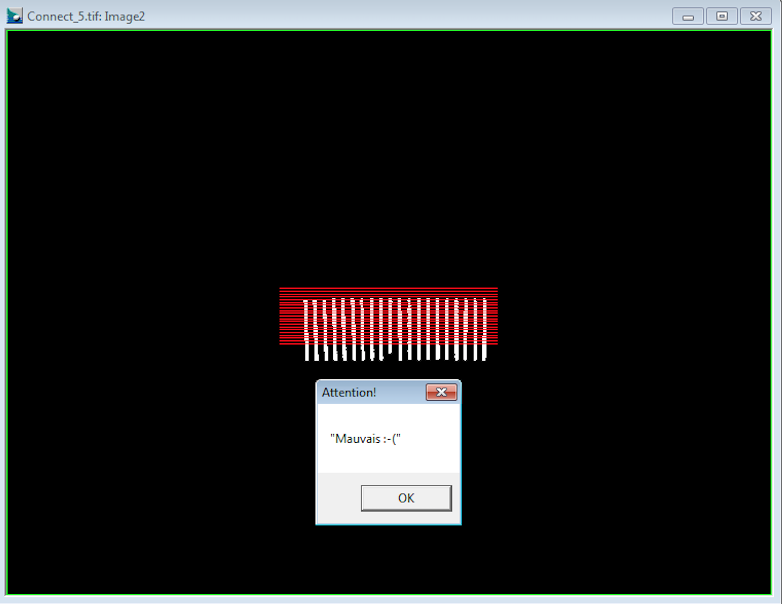
\includegraphics[width=5cm, height=5cm]{images/connecteur5.png}
\caption{Résultat de la macro pour l'image Connect_5.tiff}
\end{figure}

Nous constatons le même problème que celui rencontré précedemment, la solution à apporter est donc la même. 

\paragraph{Autre amélioration possible : } 
Nous avons remarqué qu'une image présente un connecteur orienté dans un autre sens que les autres.
Il serait donc important de calculé l'orientation du connecteur. Pour ce faire, nous avons réfléchi à une
idée à essayer. Sachant qu'on peut calculer l'orientation d'un bord en utilisant un filtrage de détection 
de contour comme Sobel (à la place de ne calculer que le module, on pourrait également calculer l'inclinaison 
du contour et donc avoir l'orientation générale du connecteur). Cependant, cette idée apporterait un autre soucis.
En effet, ce genre de traitement amplifie beaucoup certains bruits. Il faudrait donc s'assurer que la capture ne soit
pas bruitée avant de réaliser ce traitement avant la binarisation.   

\chapter{Identification et mesures de clés}

\paragraph{Rappel de l'énoncé du problème traité :}
Dans cette seconde partie, il faut s'imaginer qu'un industriel nous demande de pouvoir identifier les différentes clés qui
arriverait sur un tapis roulant pour les trier par la suite. Pour ce faire, nous avons de même un échantillon de capture
de différentes clés. L'objectif qui peut d'identification d'une clé qui semble compliquée peut être ici réduit à la simple
mesure de l'écartement de celle-ci. De cette manière, on pourra savoir si c'est une clé de 16 ou une clée de 12 qui défile 
sur le tapis roulant, par exemple. L'échantillon nous permet de constater qu'on peut travailler dans l'optique de faible
variation de luminosité et également travailler avec une faible variation de positionnement de l'objet sur l'image.
 
\paragraph{Stratégie adoptée :}
Afin de résoudre le problème qui nous est posé, nous nous proposons de réaliser une seconde macro qui affichera
la taille de l'écartement de la clé capturée en millimètre. Cette macro se déroulera en deux temps : la binarisation 
de l'image de manière automatique comme réalisé précédemment par la première macro de contrôle de qualité, et, la mesure
de l'écartement grâce à l'analyse d'un profil de colonne bien choisi. Attention il est important de noter qu'il faut au 
préalable réaliser un calibrage (à partir d'une image étalon fournie)  du logiciel Optimas sans lequel le rapport pixel/mm
du logiciel serait éronné. Ce calibrage doit bien entendu correspondre à la même échelle que celle utilisée lors des captures.
Une autre contrainte donc évidente de cette macro sera l'utilisation de la même échelle de capture pour chaque prise. 

Suite au calibrage d'Optimas, nous réaliserons donc l'étape de binarisation de l'image pour mettre en évidence la clé étudiée (toujours
objet en blanc sur fond en noir). De cette manière, nous pouvons beaucoup plus simplement identifier grâce à la valeur de luminance 
des pixels si un pixel représente une partie de l'objet ou du fond. Pour ce faire, nous réalisons toujours une binarisation avec un 
seuillage choisi automatiquement par l'outil auto-threshold configuré avec l'option de minimisation de la variance. C'est selon nos 
tests sur l'échantillon d'images fourni, la méthode la plus viable de calcul du seuil avec le critère de mise en valeur de la clé. 

Suite à la binarisation, nous réaliserons donc l'analyse d'un profil de colonne qui passe perpendiculairement à l'axe de symétrie 
de la "machoire" de la clé. En effet, si le profil de colonne venait à ne pas être perpendiculaire, nous ne prendrions pas la mesure 
de l'écartement de la clé mais simplement une "corde" possible. Cette valeure ne serait pas très pertinante dans notre intérêt. 
Nous avons donc choisi arbitrairement deux points de l'image contenant la clé de 16 de telle manière à ce que nos deux critères soient respectés
(perpendicularité et traverssement des deux parties représentant la "machoire" de la clé). Ensuite, pour chaque pixel du profil de colonne réalisé, 
nous avons réalisé un système de conditions afin de pouvoir compter combien de pixels appartiennant au fond réprésentent l'écartement de la clé. 
En connaissant au préalable le rapport pixel/mm (ou mm/pixel) après calibrage, nous avons pu en déduire simplement une mesure en millimètre de
l'écartement de la clé. En l'occurrence, il suffisait de diviser par deux le nombre de pixel pour avoir une approximation précise au millimètre près 
de la mesure de l'écartement.    

Je rappelle enfin que de la même manière que dans la première partie, nous avons cherché à réaliser une macro simple dans un premier temps
afin d'analyser quels autres problèmes se posent, de les analyser et de les résoudre pour optenir un algorithme plus robuste. 

Nous allons donc voir dans la prochaine partie les résultats obtenus par la seconde macro (présente en annexes). 

\paragraph{Analyse des résultats obtenu avec cette seconde macro : }

Voici les résultats en image de l'exécution de la seconde macro : 

\begin{figure}[!h]
\centering
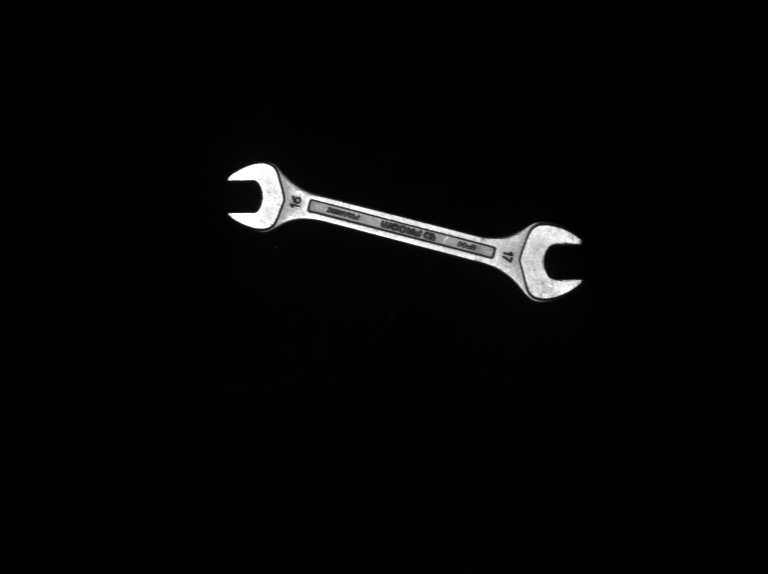
\includegraphics[width=5cm, height=5cm]{images/key1617.png}\hfill
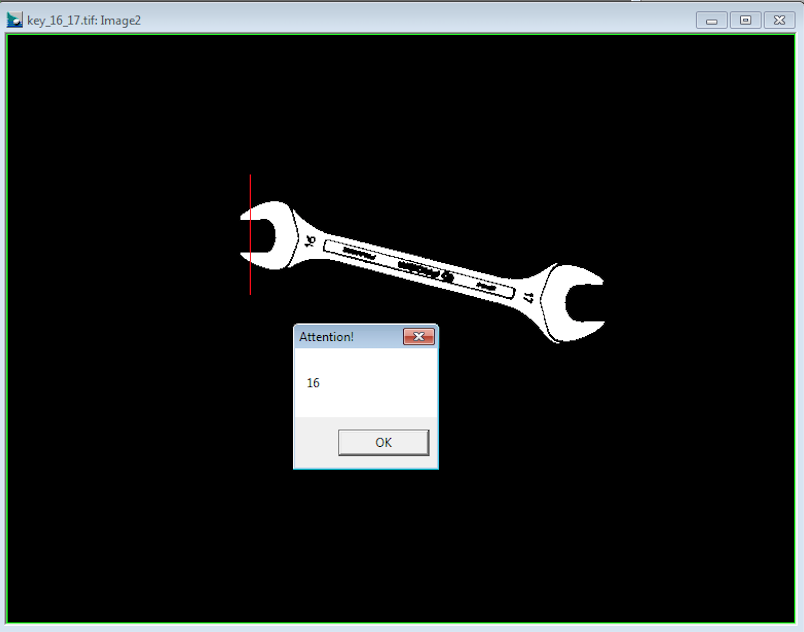
\includegraphics[width=5cm, height=5cm]{images/key16.png}
\caption{Résultat de la macro pour l'image key_16_17.tif}
\end{figure}

On observe que pour cette première image, la fonction réalise bien l'objectif souhaité. 
On remarquera la même chose pour la plupart des autres résultats.

\begin{figure}[!h]
\centering
\includegraphics[width=5cm, height=5cm]{images/key2022.png}\hfill
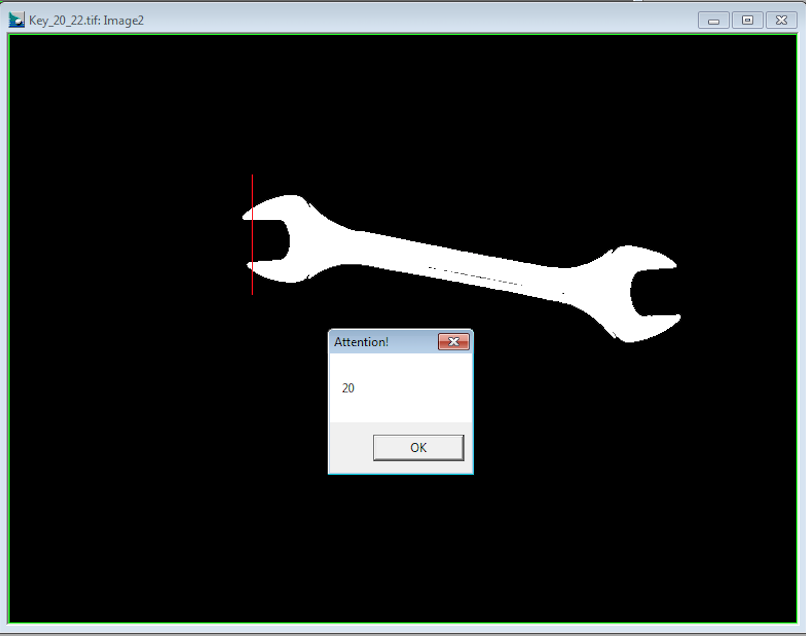
\includegraphics[width=5cm, height=5cm]{images/key20.png}
\caption{Résultat de la macro pour l'image key_20_22.tif}
\end{figure}

\newpage
\begin{figure}[!h]
\centering
\includegraphics[width=5cm, height=5cm]{images/key1415.png}\hfill
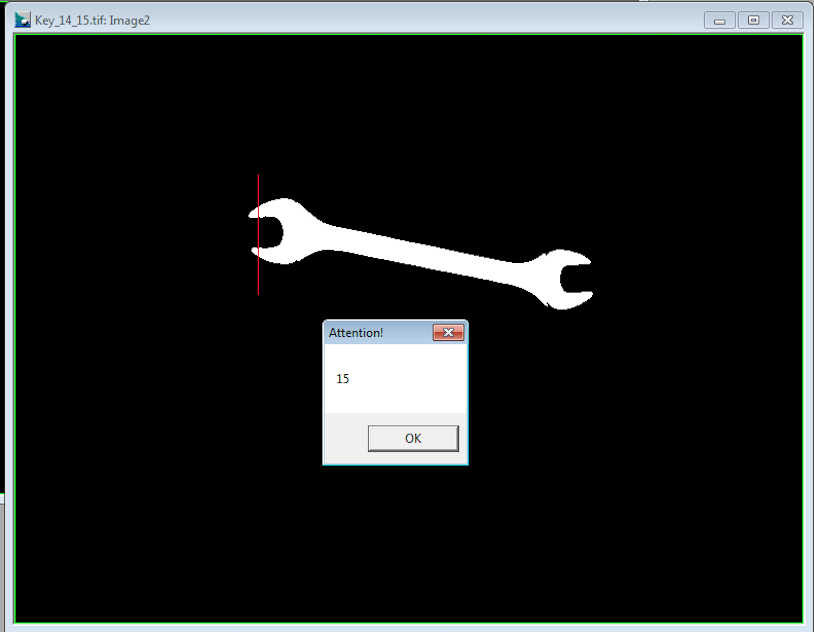
\includegraphics[width=5cm, height=5cm]{images/key15.png}
\caption{Résultat de la macro pour l'image key_14_15.tif}
\end{figure}

\begin{figure}[!h]
\centering
\includegraphics[width=5cm, height=5cm]{images/key1213.png}\hfill
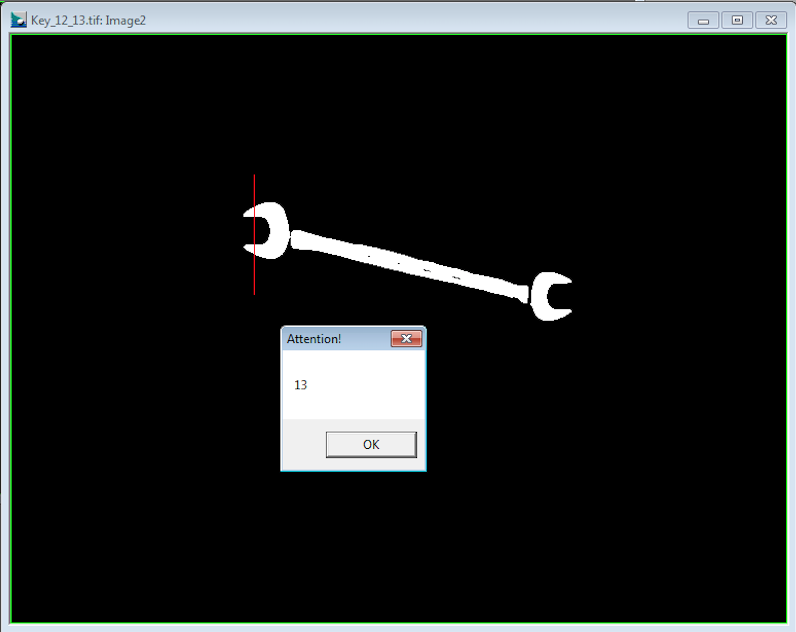
\includegraphics[width=5cm, height=5cm]{images/key13.png}
\caption{Résultat de la macro pour l'image key_12_13.tif}
\end{figure}

\begin{figure}[!h]
\centering
\includegraphics[width=5cm, height=5cm]{images/key89.png}\hfill
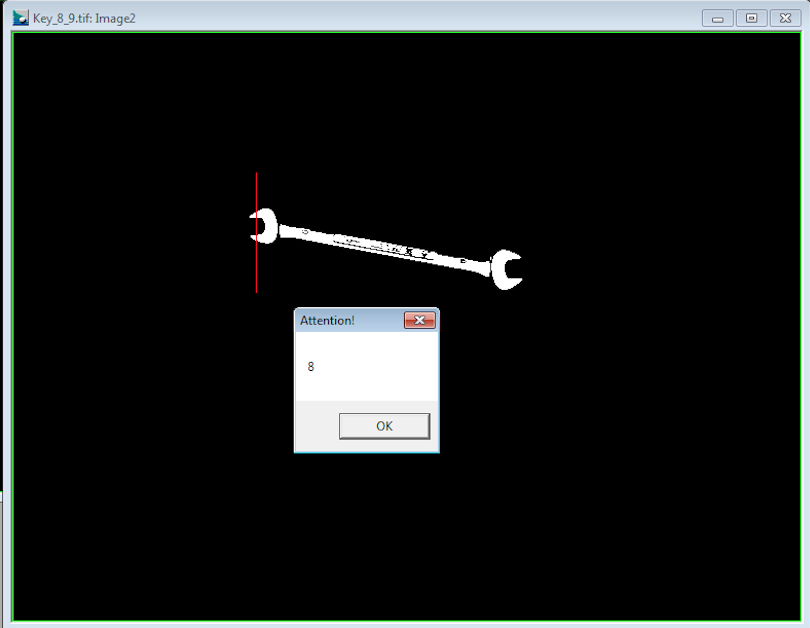
\includegraphics[width=5cm, height=5cm]{images/key8.png}
\caption{Résultat de la macro pour l'image key_8_9.tif}
\end{figure}

\newpage
Nous allons analyser maintenant les résultats obtenus avec la macro pour les images prises avec une faible luminosité et
forte luminosité.

\begin{figure}[!h]
\centering
\includegraphics[width=5cm, height=5cm]{images/key1617D.png}\hfill
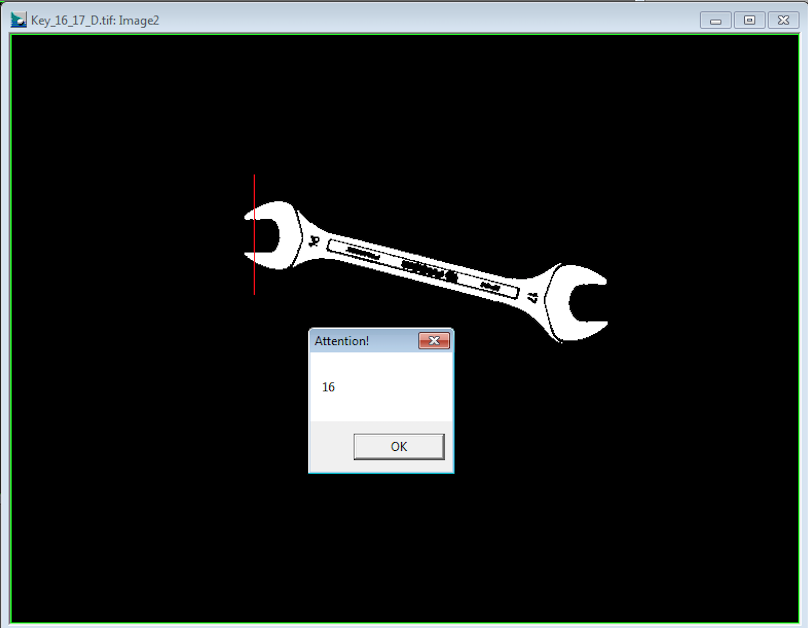
\includegraphics[width=5cm, height=5cm]{images/key16dark.png}
\caption{Résultat de la macro pour l'image key_16_17_D.tif}
\end{figure}

\begin{figure}[!h]
\centering
\includegraphics[width=5cm, height=5cm]{images/key1617L.png}\hfill
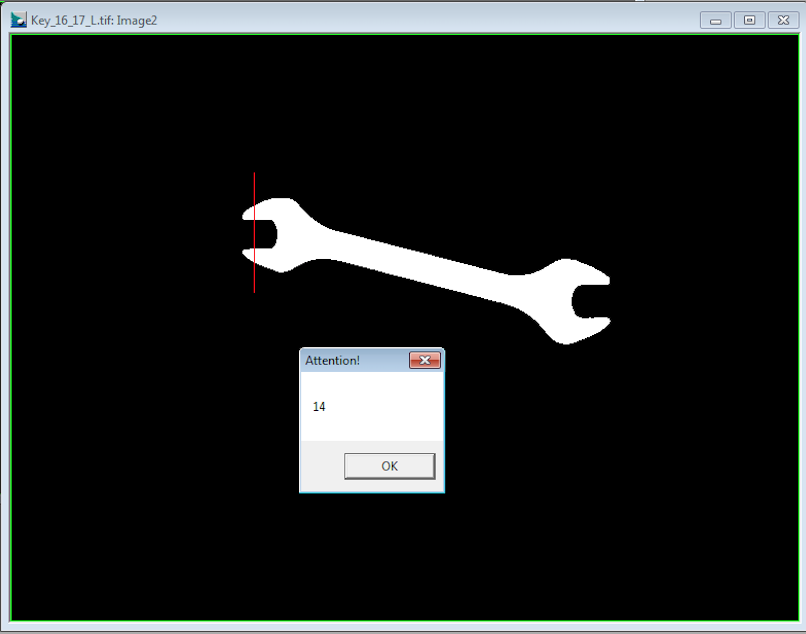
\includegraphics[width=5cm, height=5cm]{images/key16light.png}
\caption{Résultat de la macro pour l'image key_16_17_L.tif}
\end{figure}

Le résultat est bon pour l'image sombre et fausse pour l'image fortement éclairée comme supposé plus précédemment.

\chapter{Annexes}

\section{Première Macro : Contrôle qualité des connecteurs}

\begin{figure}[!h]
\centering
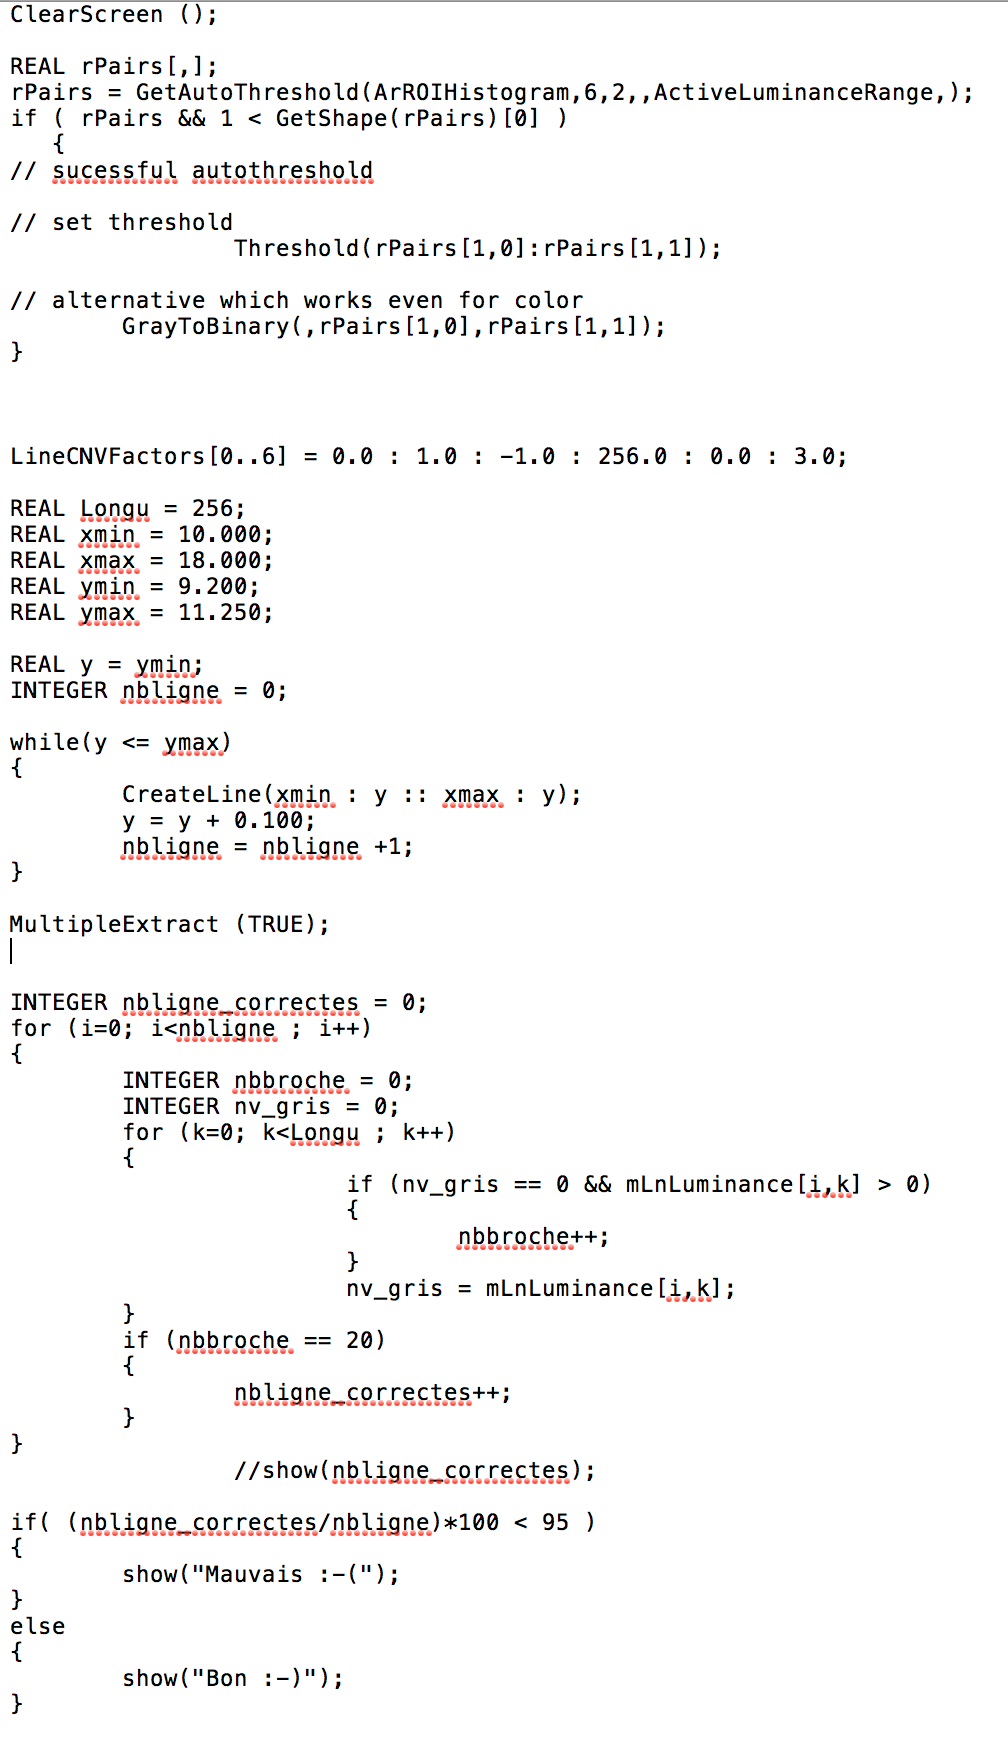
\includegraphics[width=10cm, height=15cm]{images/first.png}
\caption{Première macro de contrôle de la qualité des connecteurs}
\end{figure}


\newpage
\section{Seconde Macro : identifications et mesures de clés}

\begin{figure}[!h]
\centering
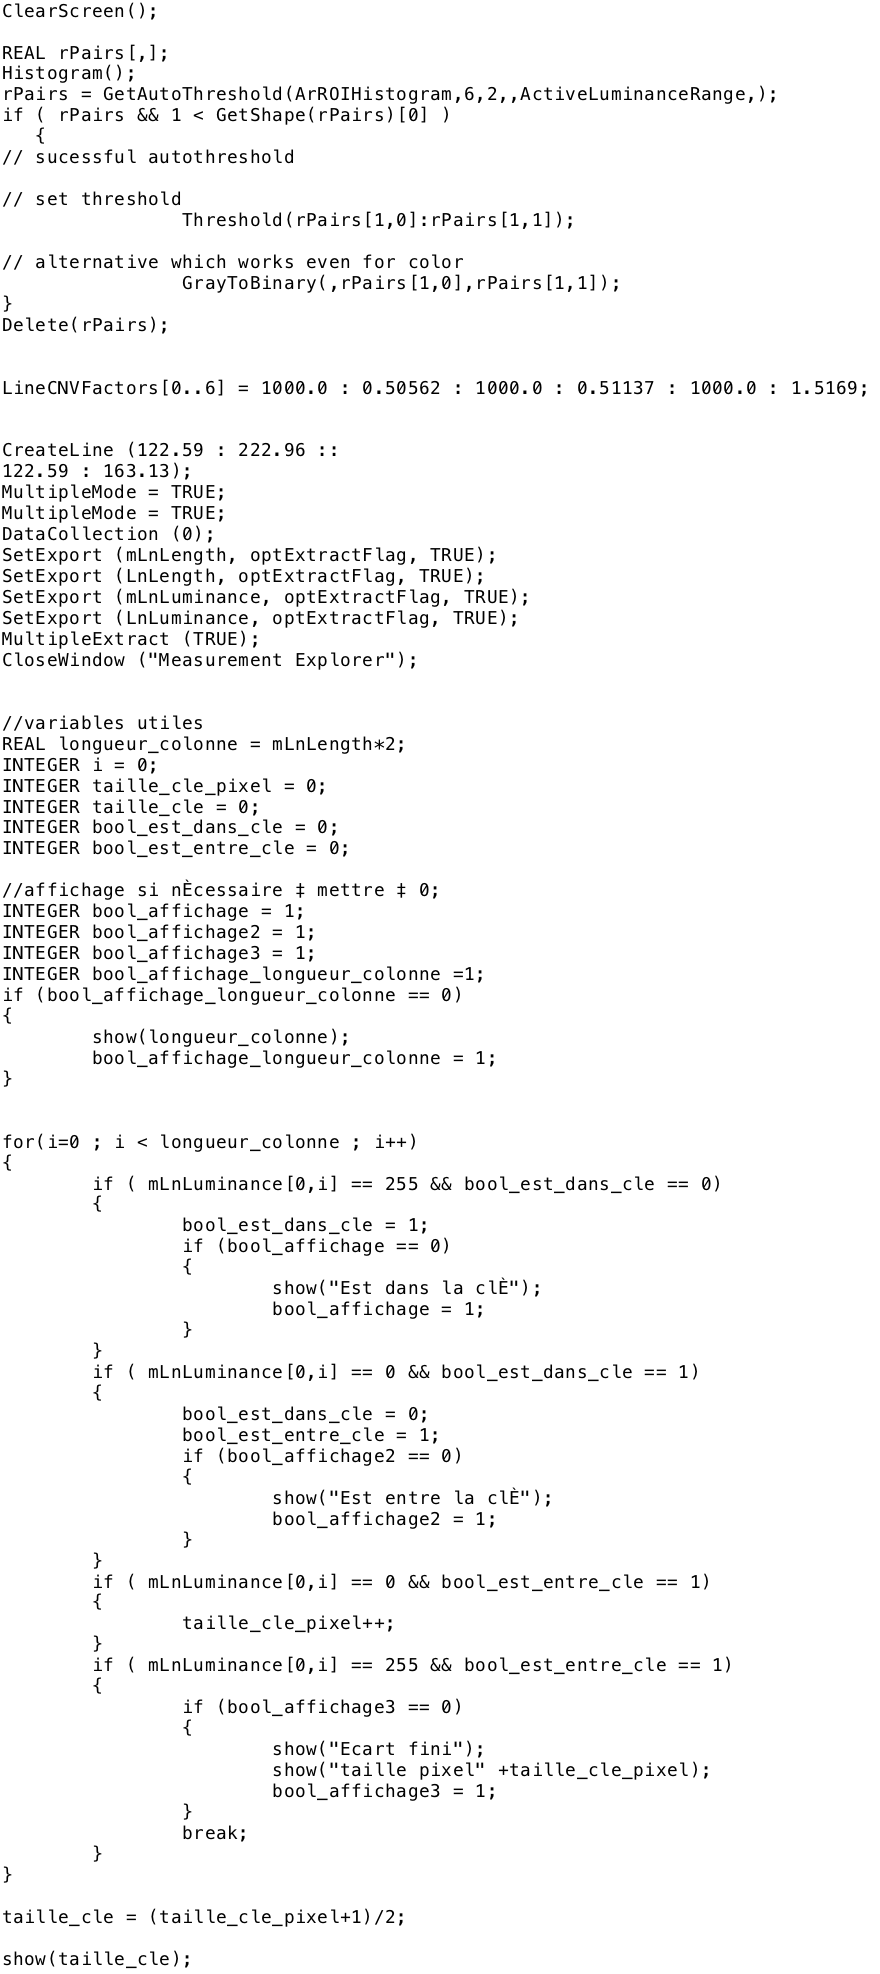
\includegraphics[width=10cm, height=18.5cm]{images/second.png}
\caption{Première macro de caractérisation des clés par leur taille}
\end{figure}

\end{document}

